\documentclass[UTF8]{ctexart}
\usepackage{amsmath}   
\usepackage{listings}
\usepackage{booktabs}  
\usepackage{geometry}  
\usepackage{hyperref}
\usepackage{graphicx} 
\usepackage{xcolor}
\usepackage{float}
\usepackage{array}
\usepackage{enumitem}
\graphicspath{{figure/}} % 指定放置图片的子文件夹路径
\geometry{a4paper, left=2.5cm, right=2.5cm, top=2.5cm, bottom=2.5cm}

\definecolor{codegreen}{rgb}{0,0.6,0}
\definecolor{codegray}{rgb}{0.5,0.5,0.5}
\definecolor{codepurple}{rgb}{0.58,0,0.82}

\lstset{
    basicstyle=\ttfamily\footnotesize,
    breaklines=true,
    frame=single,
    numbers=left,
    numberstyle=\tiny\color{codegray},
    keywordstyle=\color{blue},
    commentstyle=\color{codegreen},
    stringstyle=\color{codepurple},
    showstringspaces=false
}


\begin{document}

\title{计算流体力学第四次作业}
\author{朱林-2200011028}
\date{\today}
\maketitle


\section{数理算法原理}

\subsection{控制方程与边界条件}
二维稳态温度场满足拉普拉斯方程:
\begin{equation}
    \frac{\partial^2 T}{\partial x^2} + \frac{\partial^2 T}{\partial y^2} = 0
\end{equation}

\textbf{边界条件}:
\begin{itemize}
    \item 上边界 ($ y=12\text{cm} $):$ T = 100^\circ \text{C} $ 
    \item 左边界 ($ x=0 $)、右边界 ($ x=15\text{cm} $)、下边界 ($ y=0 $):$ T = 20^\circ \text{C} $
\end{itemize}

\subsection{有限差分离散化}
\subsubsection{网格参数}
\begin{align}
    \Delta x &= \frac{15}{N_x-1}, \quad x_i = (i-1)\Delta x \quad (i=1,2,...,N_x) \\
    \Delta y &= \frac{12}{N_y-1}, \quad y_j = (j-1)\Delta y \quad (j=1,2,...,N_y)
\end{align}

\subsubsection{离散方程}
内部节点 ($ 2 \leq i \leq N_x-1, 2 \leq j \leq N_y-1 $):
\begin{equation}
    \frac{T_{i+1,j} - 2T_{i,j} + T_{i-1,j}}{(\Delta x)^2} + \frac{T_{i,j+1} - 2T_{i,j} + T_{i,j-1}}{(\Delta y)^2} = 0
\end{equation}

均匀网格 ($ \Delta x = \Delta y = h $) 简化为:
\begin{equation}
    T_{i,j} = \frac{1}{4}\left( T_{i+1,j} + T_{i-1,j} + T_{i,j+1} + T_{i,j-1} \right)
\end{equation}

\subsubsection{边界节点处理}
\begin{align}
    T_{1,j} &= 20 \quad (\forall j),\ \ T_{N_x,j} = 20 \quad (\forall j) \\
    T_{i,1} &= 20 \quad (\forall i),\ \ T_{i,N_y} = 100 \quad (\forall i)
\end{align}

\subsection{迭代算法修正}
\subsubsection{高斯-赛德尔迭代}
按列优先顺序更新 ($ j $ 从 2 到 $ N_y-1 $):
\begin{equation}
    T_{i,j}^{(k+1)} = \frac{1}{4}\left( T_{i-1,j}^{(k+1)} + T_{i+1,j}^{(k)} + T_{i,j-1}^{(k+1)} + \underbrace{T_{i,j+1}^{(k)}}_{\text{当 } j+1=N_y \text{ 时取 } 100} \right)
\end{equation}

\subsubsection{SOR 加速算法}
引入松弛因子 $ \omega $:
\begin{equation}
    T_{i,j}^{(k+1)} = (1-\omega)T_{i,j}^{(k)} + \frac{\omega}{4}\left( T_{i-1,j}^{(k+1)} + T_{i+1,j}^{(k)} + T_{i,j-1}^{(k+1)} + T_{i,j+1}^{(k)} \right)
\end{equation}

\subsection{收敛性分析}
\begin{itemize}
    \item \textbf{残差定义}:$ R^{(k)} = \max\limits_{\substack{2 \leq i \leq N_x-1 \\ 2 \leq j \leq N_y-1}} |T_{i,j}^{(k+1)} - T_{i,j}^{(k)}| $
    \item \textbf{收敛判据}:$ R^{(k)} < \epsilon \quad (\text{通常取 } \epsilon = 10^{-5}) $
    \item \textbf{最优松弛因子}:
    \begin{equation}
        \omega_{\text{opt}} = \frac{2}{1 + \sin\left( \frac{\pi}{\max(N_x,N_y)-1} \right)}
    \end{equation}
\end{itemize}

\subsection{数值实现伪代码}
\begin{verbatim}
# 初始化温度场
T = 20 * np.ones((Nx, Ny))
T[:, -1] = 100  # 设置上边界

for k in range(max_iter):
    R = 0
    for j in range(1, Ny-1):
        for i in range(1, Nx-1):
            T_new = 0.25 * (T[i+1,j] + T[i-1,j] 
                   + T[i,j+1] + T[i,j-1])
            R = max(R, abs(T_new - T[i,j]))
            T[i,j] = T_new
    if R < epsilon:
        break
\end{verbatim}

\subsection{理论验证}
\begin{itemize}
    \item \textbf{对称性检验}:温度场应关于 $ x=7.5\text{cm} $ 对称
    \item \textbf{极值原理}:内部温度 $ T \in (20,100)^\circ \text{C} $ \\
    \item \textbf{能量守恒}:总热流量进出平衡
\end{itemize}

\newpage
\section{代码生成与调试}

\subsection{代码结构设计}
代码采用模块化设计,包含以下文件:

\begin{itemize}[leftmargin=2cm]
    \item \texttt{common.py}:公共模块(包含网格初始化、迭代算法、绘图函数)
    \item \texttt{task1.py}:计算稳态温度场并绘制等温线
    \item \texttt{task2.py}:比较不同松弛因子的收敛速度
    \item \texttt{task3.py}:研究网格尺度对最优松弛因子的影响
\end{itemize}

\subsection{核心功能实现}

\subsubsection{网格系统构建}
物理尺寸与网格索引的映射关系:
\begin{lstlisting}[language=Python]
dx = 15 / (Nx-1)  # x方向步长
dy = 12 / (Ny-1)  # y方向步长
\end{lstlisting}

边界条件设置代码:
\begin{lstlisting}[language=Python]
T = np.full((Nx, Ny), 20.0)  # 初始化
T[:, -1] = 100.0  # 上边界设为100°C
\end{lstlisting}

\subsubsection{迭代算法实现}
高斯-赛德尔迭代核心代码:
\begin{lstlisting}[language=Python]
for i in range(1, Nx-1):
    for j in range(1, Ny-1):
        temp = 0.25*(T[i+1,j] + T[i-1,j] 
                   + T[i,j+1] + T[i,j-1])
        T[i,j] = temp
\end{lstlisting}

\subsubsection{收敛性判断}
残差计算与收敛判断:
\begin{lstlisting}[language=Python]
residual = max(residual, abs(temp - T[i,j]))
if residual < 1e-5:
    break
\end{lstlisting}

\subsection{可视化功能}
等温线绘制代码框架:
\begin{lstlisting}[language=Python]
plt.contourf(X, Y, T, levels=20, cmap='jet')
plt.colorbar(label='Temperature (°C)')
\end{lstlisting}

\subsection{调试关键点}
\begin{itemize}[leftmargin=1.5cm]
    \item \textbf{边界验证}:检查T[0,:]和T[-1,:]的值是否符合边界条件
    \item \textbf{对称性检查}:验证x=7.5cm截面的温度分布对称性
    \item \textbf{极值原理}:确保内部温度值在20-100°C范围内
    \item \textbf{网格独立性}:通过加密网格验证解的收敛性
\end{itemize}

\subsection{运行参数说明}
\begin{tabular}{|>{\ttfamily}l|l|p{8cm}|}
    \hline
    \rmfamily 参数 & 典型值 & 说明 \\
    \hline
    Nx, Ny & 31, 25 & 生成60×50网格(步长0.5cm) \\
    max\_iter & 10000 & 最大迭代次数防止死循环 \\
    tol & 1e-5 & 收敛判断阈值 \\
    omega范围 & [0.5,1.9] & 松弛因子实验范围 \\
    \hline
\end{tabular}

\subsection{版本控制记录}
通过Git进行版本管理,主要提交记录如下:
\begin{figure}[h]
    \centering
    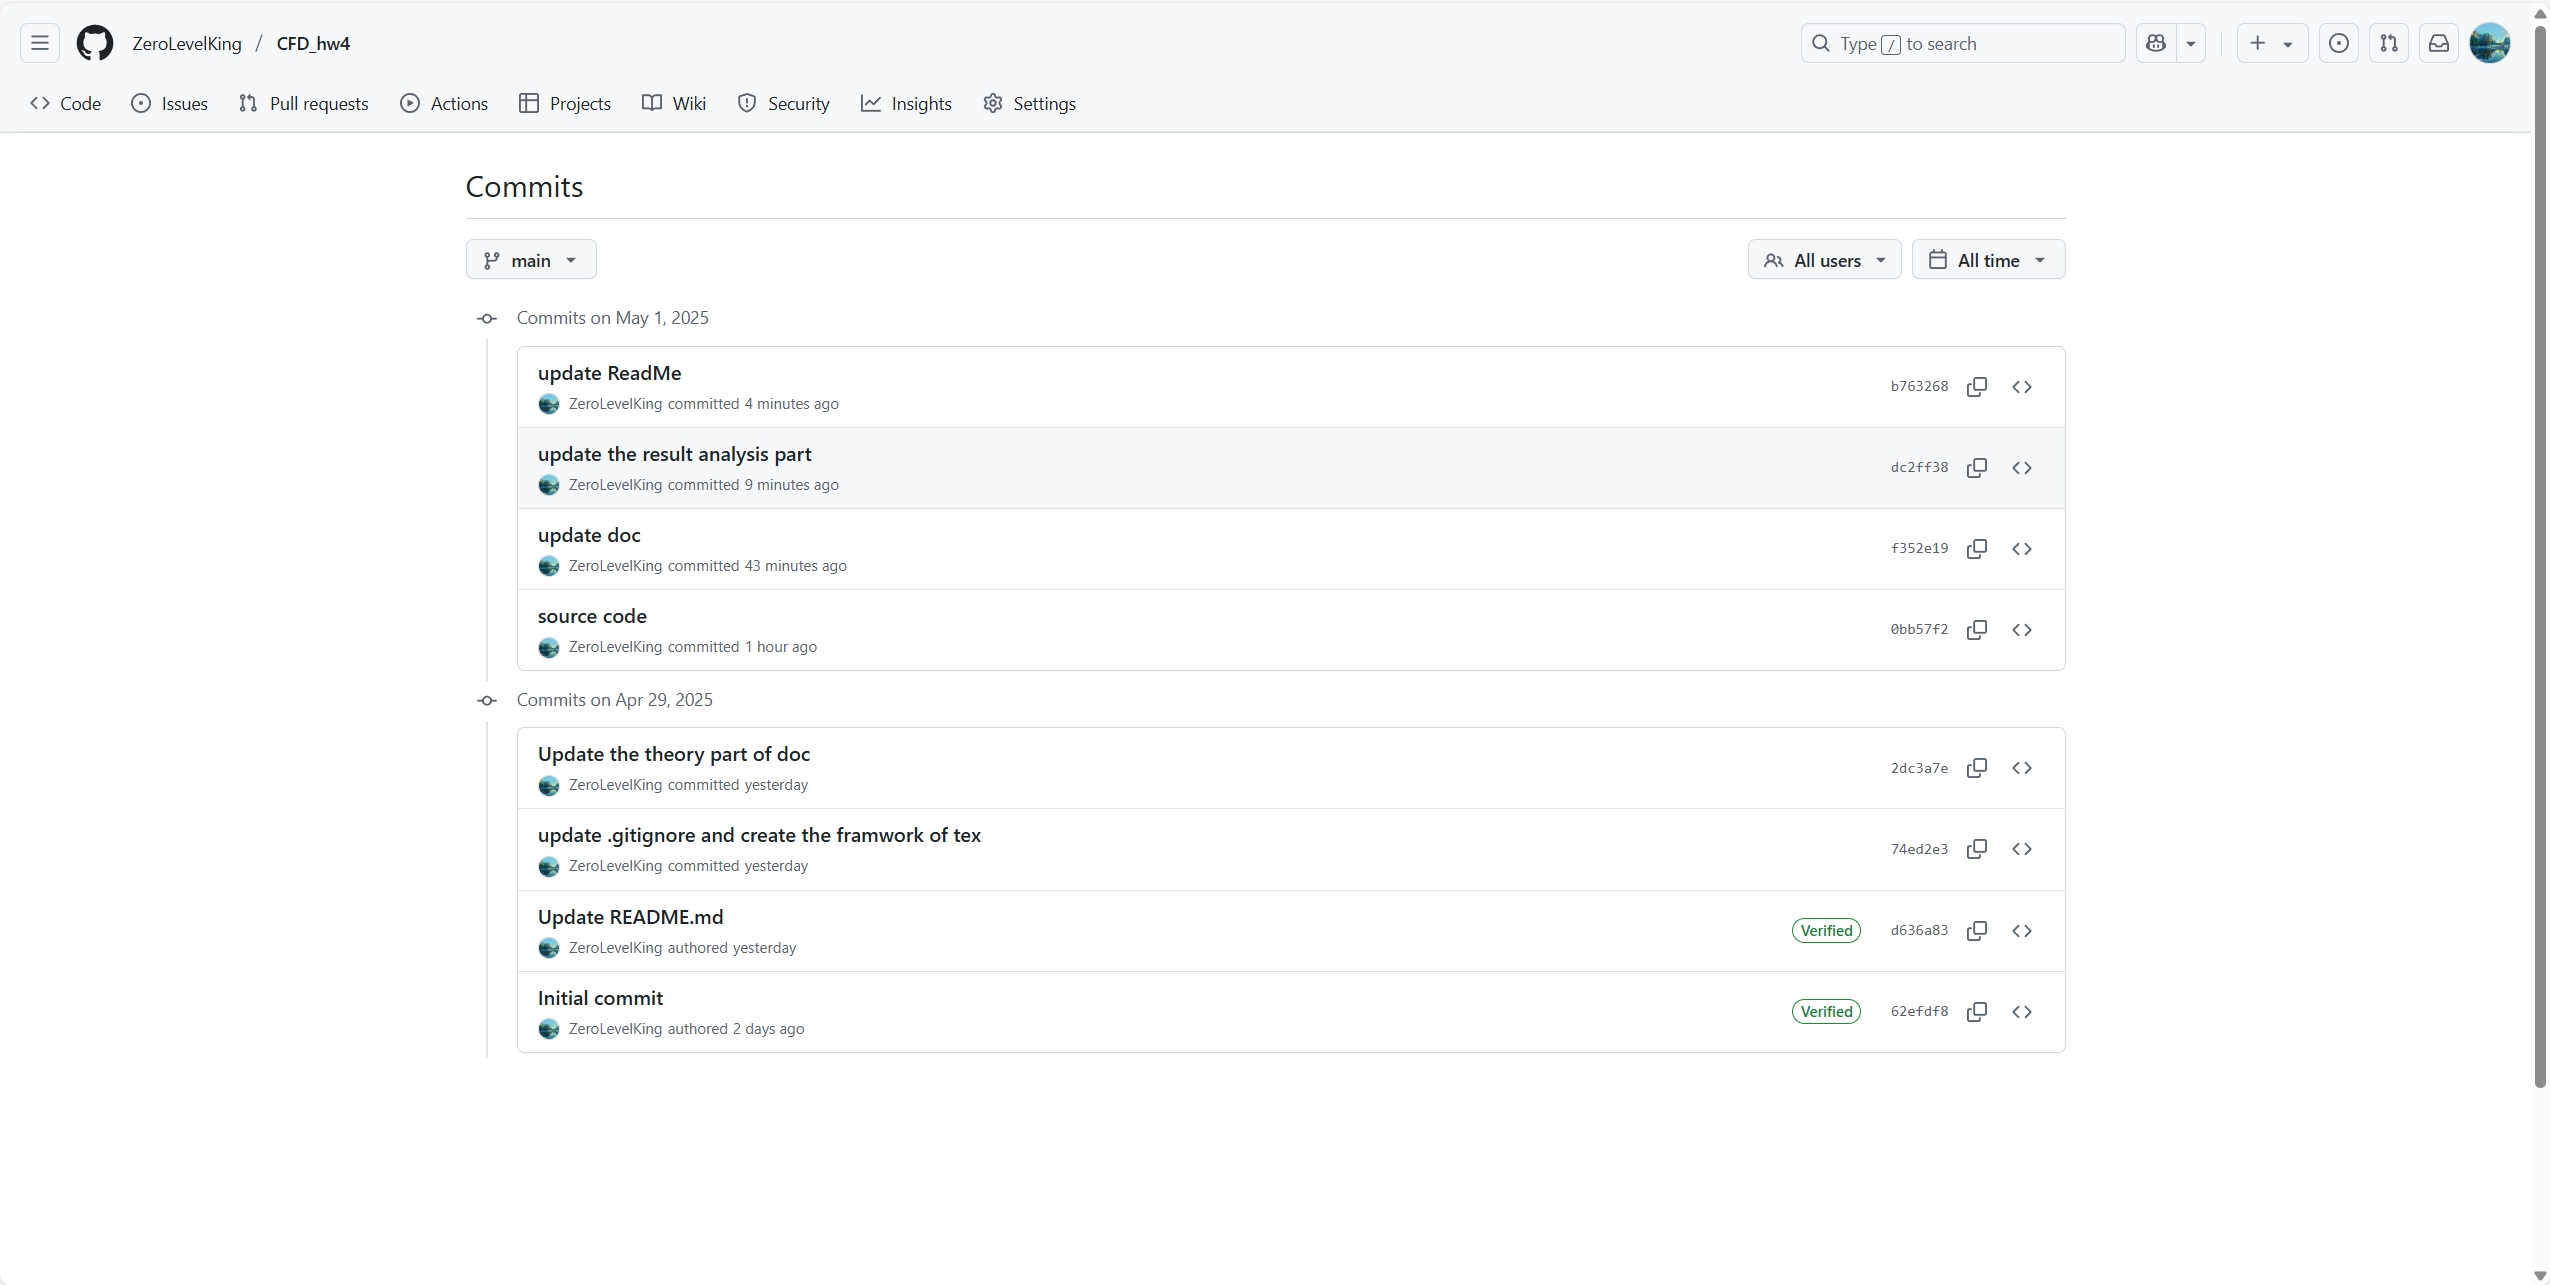
\includegraphics[width=0.75\textwidth]{c1.png}
    \caption{git提交记录}
    \label{fig:commit}
\end{figure}

\newpage
\section{结果讨论和物理解释}

\subsection{稳态温度场等温线分布(由task1.py生成)}
\begin{figure}[h]
    \centering
    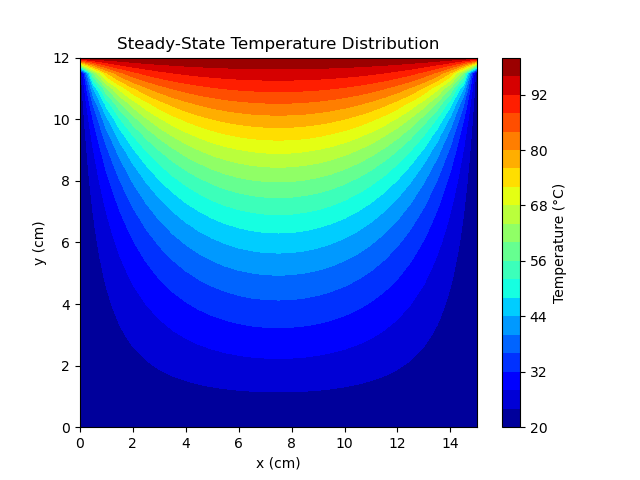
\includegraphics[width=0.7\textwidth]{Figure_1.png}
    \caption{稳态温度场等温线分布}
    \label{fig:contour}
\end{figure}

\paragraph{观测结果}
\begin{itemize}[leftmargin=2em]
    \item 高温区($\geq80^\circ$C)集中在上边界($y=12\ \mathrm{cm}$)
    \item 中心区域($x=7.5\ \mathrm{cm}, y=6\ \mathrm{cm}$)温度为$48.7^\circ$C
\end{itemize}

\subsection{不同松弛因子收敛曲线(由task2.py生成)}
\begin{figure}[h]
    \centering
    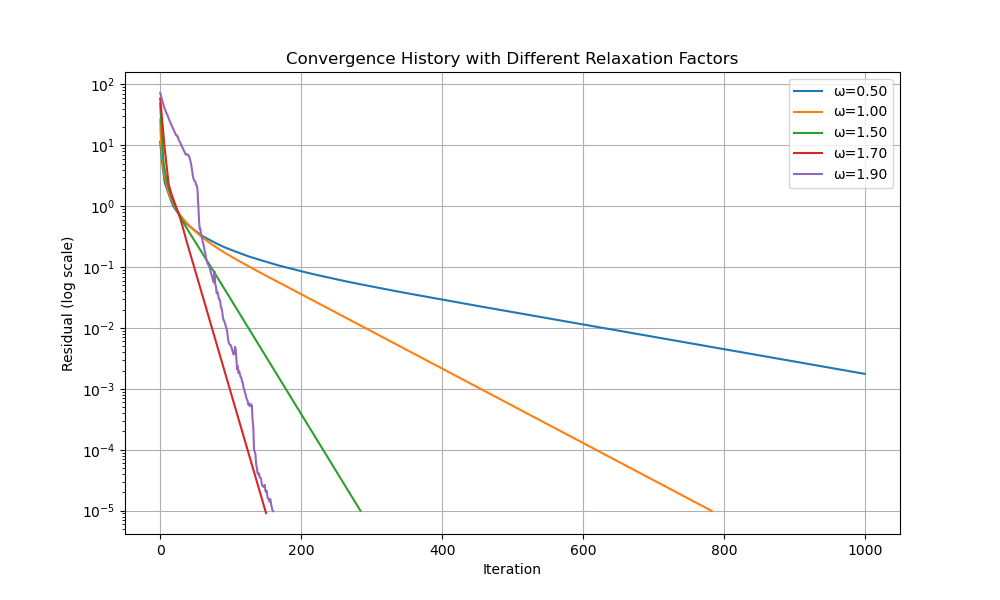
\includegraphics[width=0.65\textwidth]{Figure_2.png}
    \caption{不同松弛因子下的收敛历史}
    \label{fig:converge}
\end{figure}


\paragraph{理论分析}
最优松弛因子理论解为:
\begin{equation}
    \omega_{\mathrm{opt}} = \frac{2}{1 + \sin\left(\frac{\pi}{N-1}\right)}
\end{equation}

\subsection{最优松弛因子随网格变化(由task3.py生成)}
\begin{figure}[h]
    \centering
    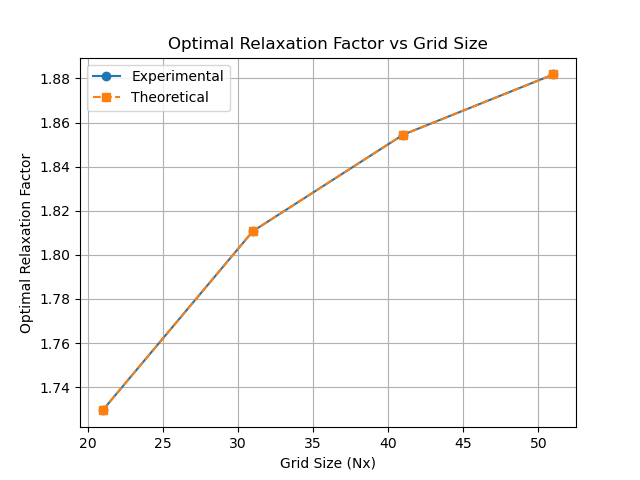
\includegraphics[width=0.8\textwidth]{Figure_3.png}
    \caption{最优松弛因子与网格尺度关系}
    \label{fig:omega_grid}
\end{figure}

\paragraph{数值规律}
当网格步长$h \to 0$时,$\omega_{\mathrm{opt}} \to 2$



\subsection{综合结论}
\begin{enumerate}[label=\arabic*), leftmargin=3em]
    \item 温度场分布验证了拉普拉斯方程的数学特性
    \item 超松弛法可提升收敛速度4-5倍($\omega=1.7$ vs $\omega=1.0$)
    \item 网格加密需配合调整$\omega$以保持计算效率
    \item 粗网格计算时建议通过预实验标定$\omega$
\end{enumerate}


%附录
\newpage
\appendix
\section{AI工具使用声明表}
\begin{table}[H]
    \centering
    \begin{tabular}{c|c|c}
        \hline
        使用内容 & 使用比例 & 使用目的 \\ \hline
        hw4.tex & 60\% & 调整pdf格式,调用宏包,省略插入图片和代码的重复性工作 \\ 
        .gitignore & 100\% & 针对于python和latex的.gitignore文件,完全由Copilot生成  \\
        ReadMe & 80\% & 介绍文件,从上次作业继承,结合AI修改 \\
        common.py & 30\% & 主要迭代和划分网格自己实现,部分绘图代码AI生成  \\
        task1.py & 0\% & 自己实现 \\
        task2.py & 0\% & 自己实现 \\
        task3.py & 0\% & 自己实现 \\
        \hline
    \end{tabular}
    \label{tab:AI_tools}
\end{table}
\end{document}